\section{Proof of testing}

In order to test the performance of our application, we implemented a little feature that displays the response time of Google Maps servers to process our requests. We looked at this response time with a growing number of intermediate points to visit. \textsc{Figure} \ref{fig:response} shows the results of this little experiment.
\begin{figure}[h!]
	\centering
	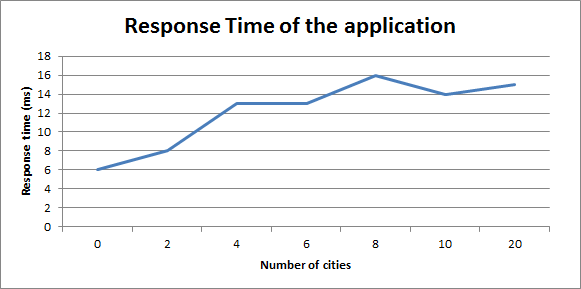
\includegraphics[scale=0.7]{input/response.png}
	\caption{Response time according to the number of points to visit.}
	\label{fig:response}
\end{figure}

\newpage As you can see, the response time does not change much, going from 6 to 16ms, which is quick enough to assure a good user experience.
We deduced from this experiment that the response time is not much influenced by the number of steps, allowing the user to organize a huge city tour.

\section{Conclusion}
			Finally, we designed a web application that allows us to personalize a city tour using the Google Maps API and JavaScript language. This tour is organized and optimized, like a human would try to do. Its instructions and the map make the way clear and it's easy to follow the instructions to reach each place you want to visit.